\documentclass[11pt,a4paper]{article}
\usepackage[utf8]{inputenc}
\usepackage{amsmath}
\usepackage{amsfonts}
\usepackage{amssymb}
\usepackage{graphicx}
\usepackage{booktabs}
\usepackage{multirow}
\usepackage{array}
\usepackage{caption}
\usepackage{subcaption}
\usepackage{xcolor}
\usepackage{colortbl}
\usepackage{siunitx}
\usepackage[margin=1in]{geometry}
\usepackage{hyperref}
\usepackage{float}
\usepackage{pgfplots}
\pgfplotsset{compat=1.18}
\hypersetup{colorlinks=true, linkcolor=blue, urlcolor=blue}

\title{Chapter X: Augmentation Experiments and Ablation Evaluation}
\author{Azizullah Massomy}
\date{\today}

\begin{document}

\maketitle

\begin{abstract}
This chapter documents the augmentation experiments I carried out for the DEEP-Dari emotion classifier. I started from a pseudo-labeled corpus of roughly 400K Dari social media posts, where Fear accounted for only 0.28\% of all examples. Under that distribution, even strong class weighting could not lift Fear F1 above 0.503.

I addressed the imbalance through a stepwise ablation study (A0--A5), a back-translation comparison (A5), and confidence-threshold experiments. Template augmentation gave the best results: run A4 reached 86.12\% accuracy and 0.857 Macro-F1, with Fear F1 rising to 0.950. Back-translation (A5) was slightly lower at 85.94\% and 0.853 Macro-F1. I also tested confidence-based label filtering: C1 (confidence $\geq 0.7$) collapsed to 75.56\% accuracy and 0.248 Fear F1 on the fixed unfiltered holdout, so I stopped before C2 and C3. Augmentation clearly beat filtering. I verify A4 stability with five training seeds (41--45) on the fixed split; results are in Table~\ref{tab:multiseed}.
\end{abstract}

\tableofcontents
\newpage

% ====================================================================
\section{Chapter Introduction}
% ====================================================================

I built DEEP-Dari to classify Afghan Persian (Dari) social media text into eight emotions: Hope, Happy, Neutral, Surprise, Disgust, Sad, Anger, and Fear. Security-related discourse in Afghanistan often carries Fear, but that class is almost invisible in large pseudo-labeled corpora. In my training set (A0), only 1,097 of 391,691 rows were labeled Fear---about 0.28\%. The baseline model still reached 85.29\% accuracy, yet Fear F1 stayed at 0.503 even with a 357$\times$ class weight.

This chapter asks three research questions:

\begin{enumerate}
    \item \textbf{RQ1:} Can targeted augmentation improve rare-class F1 when pseudo-labels are severely imbalanced?
    \item \textbf{RQ2:} Does each minority augmentation (Fear, Surprise, Anger, Disgust) contribute measurably in a stepwise ablation?
    \item \textbf{RQ3:} Is augmentation more effective than (a) extreme loss weighting alone and (b) confidence-based label filtering?
\end{enumerate}

I answer RQ1 and RQ2 through the ablation study A0--A5. Run A0 tests loss weighting without augmentation; A1--A4 add templates one layer at a time; A5 adds back-translation on top of A4. I answer RQ3 by comparing A0 (weighting only) and A4 (full augmentation), and by training C1 at confidence $\geq 0.7$ on the filtered train pool with evaluation on the fixed unfiltered holdout. C1 failed badly enough that I did not run C2 or C3.

The chapter is organized as follows. Section~\ref{sec:setup} describes the training setup and evaluation protocol. Section~\ref{sec:datasets} explains how I built the ablation datasets. Sections~\ref{sec:templates} and~\ref{sec:bt} present the template and back-translation methodology. Section~\ref{sec:ablation} reports ablation results. Section~\ref{sec:confidence} covers confidence filtering. Section~\ref{sec:discussion} discusses the findings against the research questions. Section~\ref{sec:limitations} states limitations. Section~\ref{sec:summary} closes the chapter. Reproducibility commands are in Appendix~A (see \texttt{docs/appendix\_reproducibility.md}).

% ====================================================================
\section{Experimental Setup}
\label{sec:setup}
% ====================================================================

\subsection{Model and Training Configuration}

I used the same training configuration for all ablation and confidence experiments. I fine-tuned ParsBERT (\texttt{bert-base-parsbert-uncased}) with batch size 16, max sequence length 256, and dynamic padding. I set the learning rate to $1 \times 10^{-5}$ with linear decay and optimized with AdamW (weight decay 0.01). I trained for up to four epochs with early stopping (patience 3). I applied inverse-frequency class weights: $w_i = N_{\text{total}} / N_i$.

Table~\ref{tab:weights_progression} shows how Fear weights changed as I added augmented data. At A0, Fear received a 357$\times$ weight; after I introduced Fear templates at A1, that dropped to about 39$\times$, reflecting the change in class frequency rather than a different weighting scheme.

\begin{table}[H]
\centering
\caption{Inverse-frequency class weights across ablation datasets.}
\label{tab:weights_progression}
\begin{tabular}{@{}lcccc@{}}
\toprule
Emotion & A0 & A1 & A2 & A4 \\
\midrule
Fear     & 357.06$\times$ & 39.68$\times$ & 39.08$\times$ & 38.80$\times$ \\
Anger    &  14.71$\times$ & 14.71$\times$ & 14.88$\times$ & 11.36$\times$ \\
Surprise &  21.81$\times$ & 21.81$\times$ & 14.87$\times$ & 15.21$\times$ \\
Disgust  &  13.76$\times$ & 13.76$\times$ & 14.00$\times$ & 14.32$\times$ \\
\bottomrule
\end{tabular}
\end{table}

\subsection{Evaluation Protocol}
\label{sec:eval-protocol}

Fair comparison across experiments required a fixed evaluation protocol. I used a single 80/20 train--test split with \texttt{random\_state=42}, stratified by emotion label. The split is applied once and reused.

For ablation runs A0--A5, I trained on the full augmented dataset for each run and evaluated on the held-out 20\%. For confidence experiments, I split the pseudo-labeled base once into a train pool (313,352 rows) and a fixed holdout (78,339 rows). I applied confidence filtering only to the train pool. I always evaluated on the \textit{unfiltered} holdout.

This distinction matters. When I first trained and tested C1 on the same filtered subset at confidence $\geq 0.7$, accuracy reached 98.6\% with Macro-F1 0.972 (Table~\ref{tab:leakage}). That figure is misleading: the test set no longer matched the distribution the model would face on real unfiltered social media. I therefore report confidence results only on the fixed unfiltered holdout.

For imbalanced eight-class data, I report both accuracy and Macro-F1, and I pay particular attention to per-class F1 for minority emotions. Accuracy alone can look strong while Fear remains unlearnable.

% ====================================================================
\section{Dataset Construction}
\label{sec:datasets}
% ====================================================================

I built the ablation datasets incrementally. Table~\ref{tab:ablation_datasets} lists the final row counts, which I verified in July 2026 using an audit script. One point I want to note early: the row count does not increase at every step. A2 is smaller than A1 because my merge step removes duplicate texts.

\begin{table}[H]
\centering
\caption{Datasets used in the ablation experiments.}
\label{tab:ablation_datasets}
\begin{tabular}{@{}clrr@{}}
\toprule
Run & Augmentation added & Rows & Duplicate texts \\
\midrule
A0 & Pseudo-labeled base only & 391,691 & 15,215 \\
A1 & Fear templates (9,000) & 400,691 & 15,215 \\
A2 & Surprise templates (9,000), merged with dedup & 394,476 & 0 \\
A3 & Anger templates (9,000), merged with dedup & 403,476 & 0 \\
A4 & Disgust templates (9,000), merged with dedup & 412,476 & 0 \\
A5 & Back-translation (1,439 accepted), merged with dedup & 413,914 & 0 \\
\bottomrule
\end{tabular}
\end{table}

For A1, I appended 9,000 Fear samples to the base file without deduplication. From A2 onward, I normalized text (unifying ي/ی and ك/ک) and dropped duplicate sentences before writing each merged file. When I merged Surprise onto A1, 6,215 overlapping rows were removed, bringing the total from 400,691 down to 394,476. A3 through A5 grew again as I added new unique samples. I kept this behaviour rather than rebuilding A0/A1, since I had already trained the ablation models on those files.

I summarize the base class distribution for A0 in Table~\ref{tab:label_dist}. Fear is roughly a hundred times rarer than Happy.

\begin{table}[H]
\centering
\caption{Label distribution in the pseudo-labeled base dataset (A0).}
\label{tab:label_dist}
\begin{tabular}{@{}lrr@{}}
\toprule
Emotion & Count & Share \\
\midrule
Happy    & 123,222 & 31.46\% \\
Neutral  &  82,911 & 21.17\% \\
Sad      &  75,277 & 19.22\% \\
Hope     &  36,123 &  9.22\% \\
Disgust  &  28,469 &  7.27\% \\
Anger    &  26,636 &  6.80\% \\
Surprise &  17,956 &  4.58\% \\
\rowcolor{red!15}
Fear     &   1,097 &  0.28\% \\
\bottomrule
\end{tabular}
\end{table}

% ====================================================================
\section{Template Augmentation Methodology}
\label{sec:templates}
% ====================================================================

I implemented two augmentation paths. The primary one is a template engine I wrote for Fear, Surprise, Anger, and Disgust. The secondary path, described in Section~\ref{sec:bt}, uses back-translation on sentences from the 4K gold-labeled seed.

\subsection{Design Motivation}

My early template prototypes repeated the same syntactic frame too often. The classifier began to pick up surface patterns rather than emotion. In the final design, I combined several ideas from the augmentation literature. I built templates from compositional frames with slots filled from separate lexical banks (Jia \& Liang, 2016). For label-preserving noise, I used AEDA-style punctuation insertion (Karimi et al., 2021) and optional-modifier dropout adapted from EDA (Wei \& Zou, 2019). I added orthographic variation (ي/ی swaps, zero-width character handling, elongated interjections) to reflect how Dari appears on Afghan social media. I capped each frame at roughly 2.2$\times$ its fair share of the batch and reported distinct-n scores (Li et al., 2016) to guard against mode collapse. I seeded each run and logged frame counts to a JSON sidecar (Gebru et al., 2021).

Generic English emotion templates would not work here. Afghan social media Fear is tied to war, border insecurity, and political hostility; Anger targets officials and price gougers; Disgust targets corruption. I wrote the lexicons and frames as a native Dari speaker.

Table~\ref{tab:template_outputs} summarizes the template outputs. I generated 9,000 samples per emotion (36,000 total).

\begin{table}[H]
\centering
\caption{Template augmentation outputs for the ablation study.}
\label{tab:template_outputs}
\begin{tabular}{@{}lr@{}}
\toprule
Emotion & Samples \\
\midrule
Fear     & 9,000 \\
Surprise & 9,000 \\
Anger    & 9,000 \\
Disgust  & 9,000 \\
\midrule
Total    & 36,000 \\
\bottomrule
\end{tabular}
\end{table}

\subsection{Fear Templates}

Fear was the most critical class. I structured Fear generation around three themes in Afghan online discourse: war and security (55\% of samples), political hostility (25\%), and future anxiety (20\%). I filled slots from actor banks (Taliban, Pakistan, ISIS, etc.), insult lexicons, and event verbs (attack, explosion, oppression).

Example frames I used:
\begin{itemize}
    \item \textit{ای خدا رحم کن، پاکستان هر لحظه ممکن است حمله کند، خدا رحم کنه}
    \item \textit{می‌ترسم طالبان دوباره مردم را بکشند}
    \item \textit{نگران آیندهٔ کودکان هستم که همه چیز خراب‌تر شود}
\end{itemize}

Translated emotion word lists from English would miss this domain specificity. Fear in my data is not abstract worry; it is tied to named actors and security events.

\subsection{Surprise Templates}

For Surprise, I used mirativity frames---the grammar of unexpected outcomes. I built nine frame types: exclamative leads, rhetorical questions, disbelief statements, and shock narratives. Slot banks cover price shocks, political reversals, and market crashes.

Examples:
\begin{itemize}
    \item \textit{وای! قیمت‌ها یک‌شبه تغییر کرد}
    \item \textit{چطور ممکن است حکومت دوباره وعدهٔ میان‌تهی بدهد؟}
    \item \textit{باورم نمی‌شود، بازار واقعاً سقوط کرد}
\end{itemize}

\subsection{Anger Templates}

For Anger, I focused on blame assignment and collective frustration---patterns common in Afghan complaint posts. Targets include officials, hoarders, corrupt administrators, and media. Frames cover direct accusation, rhetorical challenge, and collective exhaustion.

Examples:
\begin{itemize}
    \item \textit{این مسئولین مردم را فراموش کرده‌اند}
    \item \textit{به خدا قسم، زورمندان دیگر بس است}
    \item \textit{چرا ادارهٔ برق هیچ کاری نمی‌کند؟}
\end{itemize}

\subsection{Disgust Templates}

For Disgust, I used moral revulsion and social withdrawal frames: interjection plus evaluation, normalization laments (``it has become normal''), and physical-revulsion metaphors. Slot banks target corruption, bribery, hypocrisy, and injustice.

Examples:
\begin{itemize}
    \item \textit{اف به این روزگار، این فساد اداری قابل تحمل نیست}
    \item \textit{این رشوت‌خوری در این کشور شرم‌آور است}
    \item \textit{از این دورویی بیزارم، حال آدم را بد می‌کند}
\end{itemize}

\subsection{Surface Perturbations}

After filling a frame, I applied label-preserving perturbations with fixed probabilities (Table~\ref{tab:perturbations}). These keep the emotion label intact while adding social-media realism.

\begin{table}[H]
\centering
\caption{Surface perturbations applied during template generation.}
\label{tab:perturbations}
\begin{tabular}{@{}lll@{}}
\toprule
Technique & Probability & Role \\
\midrule
Discourse prefix       & 30\% & Varied post openings \\
Discourse ending       & 22\% & Natural closings \\
AEDA punctuation       & 15\% & Typing noise \\
Emotive elongation     & 12\% & Colloquial emphasis \\
Arabic code-point swap &  8\% & Keyboard inconsistency \\
\bottomrule
\end{tabular}
\end{table}

% ====================================================================
\section{Back-Translation Methodology}
\label{sec:bt}
% ====================================================================

For A5, I tested whether NLLB round-trip paraphrases could complement template augmentation. I used \texttt{facebook/nllb-200-distilled-600M} with \texttt{pes\_Arab} $\leftrightarrow$ \texttt{eng\_Latn}. I drew source sentences only from the 4K gold-labeled file, not from generated templates, so the paraphrases stayed rooted in authentic Dari.

\subsection{Three-Step Protocol}

I ran back-translation in three steps before training A5:

\begin{enumerate}
    \item \textbf{Spot-check:} I generated 100 samples per emotion class and reviewed them manually. I checked whether the label was still correct, whether the Dari read naturally, and whether any English leaked through. I applied a stop rule: if fewer than 80\% of spot-check samples per class were label-preserving, I would not proceed to full generation.
    \item \textbf{Full generation:} I ran round-trip translation on the gold pool per emotion (targets: Surprise 2000, Anger 2000, Disgust 2000, Sad 1500, Fear 1000).
    \item \textbf{Merge:} I appended accepted BT samples onto the A4 dataset with the same deduplication step used for template merges.
\end{enumerate}

\subsection{Quality Filters}

I rejected BT outputs that failed any of the filters in Table~\ref{tab:bt_filters}. The low overall acceptance rate (16.9\%) came from the combination of small gold pools and strict filtering, not from a broken pipeline.

\begin{table}[H]
\centering
\caption{Back-translation quality filters.}
\label{tab:bt_filters}
\begin{tabular}{@{}lll@{}}
\toprule
Filter & Threshold & Reason \\
\midrule
Minimum tokens       & $< 3$ rejected           & Fragments are not usable posts \\
Length ratio         & outside 0.5--2.0         & Collapsed or inflated outputs \\
Character overlap    & $> 0.95$ rejected        & Near-copy of source \\
Exact duplicate      & normalized match         & Round-trip produced same text \\
Empty translation    & blank output             & Model failure \\
\bottomrule
\end{tabular}
\end{table}

Fear was especially constrained: I had only 124 gold Fear sentences as sources, so even a well-tuned filter could not produce a large Fear set. Table~\ref{tab:bt_stats} gives the final counts per emotion. I kept 1,439 samples in total. Merging onto A4 added a net 1,438 rows after I removed one duplicate.

\begin{table}[H]
\centering
\caption{Back-translation generation and acceptance by emotion class.}
\label{tab:bt_stats}
\begin{tabular}{@{}lrrrr@{}}
\toprule
Emotion & Target & Accepted & Acceptance rate & Gold pool \\
\midrule
Surprise & 2,000 & 324 & 16.2\% & 367 \\
Anger    & 2,000 & 240 & 12.0\% & 279 \\
Disgust  & 2,000 & 237 & 11.9\% & 272 \\
Sad      & 1,500 & 528 & 35.2\% & 656 \\
Fear     & 1,000 & 110 & 11.0\% & 124 \\
\midrule
Total    & 8,500 & 1,439 & 16.9\% & \\
\bottomrule
\end{tabular}
\end{table}

Table~\ref{tab:examples} shows sample outputs from both augmentation paths.

\begin{table}[H]
\centering
\caption{Sample outputs from template generation and back-translation.}
\label{tab:examples}
\small
\begin{tabular}{@{}p{2.2cm}p{1.5cm}p{8.5cm}@{}}
\toprule
Method & Emotion & Example \\
\midrule
Template & Fear & \textit{Ey Khoda rahm kon, Pakistan har lahze momkin ast hamle konad.} \\
Template & Surprise & \textit{Wāy! Qaymathā yek shab taghir kard.} \\
Template & Anger & \textit{In mas'ulin mardom ra faramosh kardeand.} \\
Template & Disgust & \textit{Uf, in fesād qābel-e tahamol nist.} \\
Back-trans. & Fear & \textit{Fātemeh jān fesh, ageh morāqeb bāshi ke dokhtar daryāyi nakhori...} \\
\bottomrule
\end{tabular}
\end{table}

% ====================================================================
\section{Ablation Results}
\label{sec:ablation}
% ====================================================================

In Table~\ref{tab:complete_results}, I report accuracy, Macro-F1, and Fear F1 for all six ablation runs. Table~\ref{tab:perclass_complete} gives the per-class breakdown.

\begin{table}[H]
\centering
\caption{Ablation study results.}
\label{tab:complete_results}
\begin{tabular}{@{}llcccc@{}}
\toprule
Run & Augmentation & Acc (\%) & Macro-F1 & Fear F1 & Best epoch \\
\midrule
A0 & None & 85.29 & 0.779 & 0.503 & 4 \\
A1 & Fear & 85.75 & 0.836 & 0.946 & 3 \\
A2 & Fear + Surprise & 85.52 & 0.841 & 0.946 & 4 \\
A3 & Fear + Surprise + Anger & 85.78 & 0.850 & 0.944 & 4 \\
\rowcolor{green!20}
A4 & Full template stack & 86.12 & 0.857 & 0.950 & 3 \\
\rowcolor{blue!10}
A5 & A4 + back-translation & 85.94 & 0.853 & 0.931 & 4 \\
\bottomrule
\end{tabular}
\end{table}

The largest single change came at A1. When I added 9,000 Fear templates, Fear F1 moved from 0.503 to 0.946 and Macro-F1 from 0.779 to 0.836. That result alone justified the augmentation effort: class weighting at 357$\times$ had not come close.

When I added Surprise at A2, Surprise F1 rose from 0.754 to 0.826 (+7.2\% relative). Overall accuracy dipped slightly to 85.52\%, which I attribute to the shift in training distribution. At A3, Anger F1 improved from 0.718 to 0.782 (+6.4\%) and Macro-F1 reached 0.850. At A4, Disgust F1 rose from 0.785 to 0.835 (+5.0\%) and I obtained my best overall numbers: 86.12\% accuracy, 0.857 Macro-F1, 0.950 Fear F1.

For A5, performance was close but did not exceed A4: 85.94\% accuracy, 0.853 Macro-F1, 0.931 Fear F1. Given the small BT contribution (1,439 accepted samples against 36,000 templates), I did not expect a large gain.

\begin{table}[H]
\centering
\caption{Per-class F1 scores across ablation runs.}
\label{tab:perclass_complete}
\small
\begin{tabular}{@{}lcccccc@{}}
\toprule
Emotion & A0 & A1 & A2 & A3 & A4 & A5 \\
\midrule
Hope     & 0.869 & 0.868 & 0.858 & 0.858 & 0.860 & 0.861 \\
Happy    & 0.928 & 0.928 & 0.925 & 0.925 & 0.926 & 0.926 \\
Neutral  & 0.847 & 0.851 & 0.843 & 0.842 & 0.841 & 0.842 \\
Surprise & 0.751 & 0.754 & 0.826 & 0.831 & 0.831 & 0.829 \\
Disgust  & 0.778 & 0.785 & 0.782 & 0.781 & 0.835 & 0.830 \\
Sad      & 0.839 & 0.840 & 0.838 & 0.837 & 0.836 & 0.835 \\
Anger    & 0.714 & 0.718 & 0.713 & 0.782 & 0.780 & 0.771 \\
\rowcolor{red!15}
Fear     & 0.503 & 0.946 & 0.946 & 0.944 & 0.950 & 0.931 \\
\bottomrule
\end{tabular}
\end{table}

I plot the Macro-F1 and Fear F1 trajectories in Figures~\ref{fig:macro_progression} and~\ref{fig:fear_progression}.

\subsection{Multi-seed Stability (A4)}
\label{sec:multiseed}

To check that the A4 result was not a single lucky training run, I trained A4 five times with training seeds 41--45 while keeping the stratified train--test split fixed at \texttt{random\_state=42}. Each run writes to a separate output directory (\texttt{seed\_41} through \texttt{seed\_45}); the original anchor model at \texttt{outputs/ablation/A4/} is unchanged. I aggregate metrics with \texttt{scripts/run\_multiseed.py}; the summary is saved as \texttt{multiseed\_summary.json}.

Table~\ref{tab:multiseed} reports per-seed accuracy, Macro-F1, and Fear F1 on the same held-out 20\%. Fill mean $\pm$ std from \texttt{multiseed\_summary.json} after the GPU runs complete.

\begin{table}[H]
\centering
\caption{A4 multi-seed results (fixed split, training seeds 41--45). Replace placeholders after \texttt{run\_multiseed.py --force}.}
\label{tab:multiseed}
\begin{tabular}{@{}rccc@{}}
\toprule
Training seed & Accuracy & Macro-F1 & Fear F1 \\
\midrule
41 & --- & --- & --- \\
42 & --- & --- & --- \\
43 & --- & --- & --- \\
44 & --- & --- & --- \\
45 & --- & --- & --- \\
\midrule
Mean $\pm$ std & --- & --- & --- \\
\bottomrule
\end{tabular}
\end{table}

\begin{figure}[H]
\centering
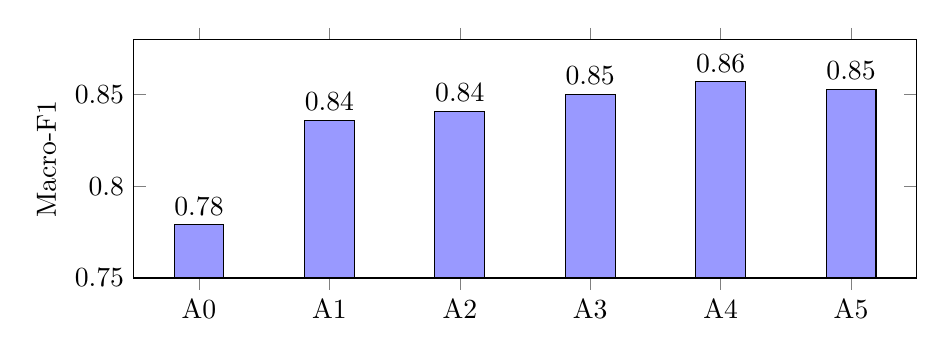
\begin{tikzpicture}
\begin{axis}[
    ybar,
    symbolic x coords={A0,A1,A2,A3,A4,A5},
    xtick=data,
    ylabel={Macro-F1},
    ymin=0.75, ymax=0.88,
    nodes near coords,
    nodes near coords align={vertical},
    width=0.95\textwidth,
    height=0.38\textwidth,
    bar width=18pt,
]
\addplot[fill=blue!40] coordinates {(A0,0.779) (A1,0.836) (A2,0.841) (A3,0.850) (A4,0.857) (A5,0.853)};
\end{axis}
\end{tikzpicture}
\caption{Macro-F1 by ablation run. A4 reaches the highest value (0.857).}
\label{fig:macro_progression}
\end{figure}

\begin{figure}[H]
\centering
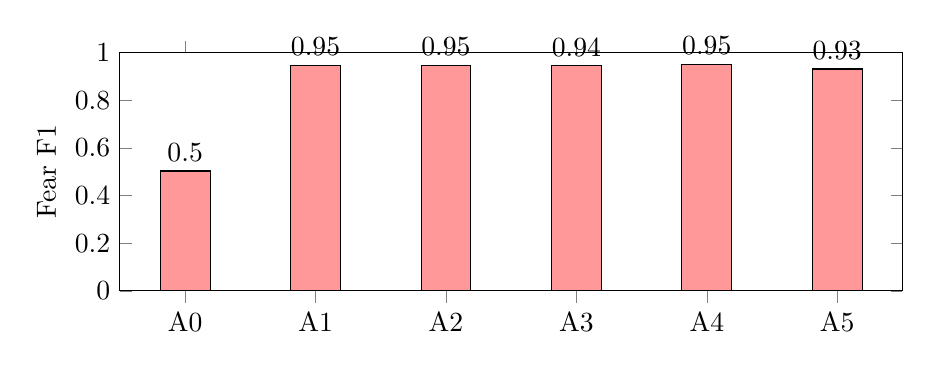
\begin{tikzpicture}
\begin{axis}[
    ybar,
    symbolic x coords={A0,A1,A2,A3,A4,A5},
    xtick=data,
    ylabel={Fear F1},
    ymin=0, ymax=1,
    nodes near coords,
    nodes near coords align={vertical},
    width=0.95\textwidth,
    height=0.38\textwidth,
    bar width=18pt,
]
\addplot[fill=red!40] coordinates {(A0,0.503) (A1,0.946) (A2,0.946) (A3,0.944) (A4,0.950) (A5,0.931)};
\end{axis}
\end{tikzpicture}
\caption{Fear F1 by ablation run. The jump occurs at A1; later runs keep Fear F1 above 0.93.}
\label{fig:fear_progression}
\end{figure}

% ====================================================================
\section{Confidence Threshold Experiments}
\label{sec:confidence}
% ====================================================================

After the ablation runs, I tested whether removing low-quality pseudo-labels could improve performance (RQ3, filtering arm). I scored all 391,691 rows with the 4K seed model, split the data into a train pool (313,352 rows) and a fixed holdout (78,339 rows), and trained \textbf{C1} on the confidence-filtered train pool at $\geq 0.7$ with label agreement required. I validated C1 on the original unfiltered holdout (Section~\ref{sec:eval-protocol}). The results were catastrophic. I stopped the confidence track after C1 and did not train C2 or C3.

\subsection{Experiment Design}

Table~\ref{tab:confidence_splits} lists the splits. C1 used 148,924 filtered training rows. I prepared C2 and C3 splits for projection analysis but never trained them.

\begin{table}[H]
\centering
\caption{Confidence experiment splits (holdout fixed at 78,339 rows).}
\label{tab:confidence_splits}
\begin{tabular}{@{}llrr@{}}
\toprule
Run & Train file & Threshold & Rows \\
\midrule
C0 & train pool (unfiltered) & ---   & 313,352 \\
C1 & train\_filtered\_conf07  & $\geq 0.7$ & 148,924 \\
C2 & train\_filtered\_conf08  & $\geq 0.8$ & 114,702 \\
C3 & train\_filtered\_conf09  & $\geq 0.9$ &  65,488 \\
\bottomrule
\end{tabular}
\end{table}

Table~\ref{tab:scoring} summarizes pseudo-label scoring. Overall agreement was 70.48\%. Anger had the lowest agreement (52.31\%); I often saw it confused with Disgust.

\begin{table}[H]
\centering
\caption{Pseudo-label scoring diagnostics.}
\label{tab:scoring}
\begin{tabular}{@{}ll@{}}
\toprule
Metric & Value \\
\midrule
Overall agreement & 70.48\% \\
Mean confidence   & 0.710 \\
Fear agreement    & 76.85\% \\
Anger agreement   & 52.31\% \\
\bottomrule
\end{tabular}
\end{table}

At the C1 threshold, retention varied widely by class (Table~\ref{tab:retention}). Anger kept only 17.3\% of its rows; Disgust kept 26.2\%. Fear survived with only 644 training samples.

\begin{table}[H]
\centering
\caption{Class retention after filtering at confidence $\geq$ 0.7 (train pool only).}
\label{tab:retention}
\begin{tabular}{@{}lrr@{}}
\toprule
Class & Original count & Retained \\
\midrule
Happy    & 123,222 & 77,240 (62.7\%) \\
Neutral  &  82,911 & 37,644 (45.4\%) \\
Sad      &  75,277 & 33,191 (44.1\%) \\
Hope     &  36,123 & 18,704 (51.8\%) \\
Disgust  &  28,469 &  7,463 (26.2\%) \\
Anger    &  26,636 &  4,616 (17.3\%) \\
Surprise &  17,956 &  6,575 (36.6\%) \\
Fear     &   1,097 &    644 (58.7\%) \\
\bottomrule
\end{tabular}
\end{table}

Filtering also shifted the label balance. Table~\ref{tab:label_skew} shows how the Happy share grows as the threshold rises. At conf $\geq 0.9$, Happy would reach 59.9\% while Anger would fall to 0.23\%.

\begin{table}[H]
\centering
\caption{Happy class share in confidence-filtered train pools (from audit).}
\label{tab:label_skew}
\begin{tabular}{@{}lrr@{}}
\toprule
Split & Threshold & Happy share \\
\midrule
Train pool (C0) & unfiltered & 31.5\% \\
C1 train          & $\geq 0.7$ & 41.5\% \\
C2 train (not run) & $\geq 0.8$ & 46.6\% \\
C3 train (not run) & $\geq 0.9$ & 59.9\% \\
\bottomrule
\end{tabular}
\end{table}

\subsection{The Data Leakage Problem}

My first C1 evaluation used a filtered test set drawn from the same high-confidence distribution as the training data. That produced artificially strong numbers (Table~\ref{tab:leakage}). When I re-evaluated on the fixed \textit{unfiltered} holdout, performance collapsed. The model had learned the filtered distribution, not the real pseudo-labeled distribution it would face in deployment.

\begin{table}[H]
\centering
\caption{C1 evaluation: filtered test set vs.\ original unfiltered holdout.}
\label{tab:leakage}
\begin{tabular}{@{}lccc@{}}
\toprule
Evaluation set & Accuracy & Macro-F1 & Fear F1 \\
\midrule
Filtered test set (invalid)     & 98.6\% & 0.972 & 0.924 \\
Original holdout (valid)        & 75.56\% & 0.648 & 0.248 \\
\bottomrule
\end{tabular}
\end{table}

This happened because the filtered subset contained only ``easy'' samples where the seed model was confident. Training and testing within that subset inflates metrics. I report only holdout results below.

\subsection{C1 Validated Performance}

On the fixed unfiltered holdout, C1 reached 75.56\% accuracy, 0.648 Macro-F1, and 0.248 Fear F1 (Table~\ref{tab:c1_results}). Compared to A4 under the same evaluation principle---generalization to real unfiltered data---the gap is large (Table~\ref{tab:c1_vs_a4}).

\begin{table}[H]
\centering
\caption{C1 results on the fixed unfiltered holdout.}
\label{tab:c1_results}
\begin{tabular}{@{}lc@{}}
\toprule
Metric & C1 \\
\midrule
\rowcolor{red!15}
Accuracy  & 75.56\% \\
\rowcolor{red!15}
Macro-F1  & 0.648 \\
Fear F1   & 0.248 \\
\bottomrule
\end{tabular}
\end{table}

\begin{table}[H]
\centering
\caption{C1 (filtered training) compared with A4 (full augmentation).}
\label{tab:c1_vs_a4}
\begin{tabular}{@{}lccc@{}}
\toprule
Metric & C1 & A4 & Difference \\
\midrule
Accuracy  & 75.56\% & 86.12\% & $-$10.56\% \\
Macro-F1  & 0.648   & 0.857   & $-$0.209 \\
Fear F1   & 0.248   & 0.950   & $-$0.702 \\
\bottomrule
\end{tabular}
\end{table}

Every emotion class performed worse under C1 than under A4 (Table~\ref{tab:per_class_c1}). Fear collapsed the most (0.950 $\rightarrow$ 0.248). Even majority classes suffered: Happy F1 fell from 0.926 to 0.874 ($-$5.2\%), and Neutral from 0.841 to 0.753 ($-$8.9\%). There was no class where filtering helped.

\begin{table}[H]
\centering
\caption{Per-class F1: A4 (augmented) vs.\ C1 (filtered), on the unfiltered holdout.}
\label{tab:per_class_c1}
\begin{tabular}{@{}lccc@{}}
\toprule
Emotion & A4 & C1 & Change \\
\midrule
Fear     & 0.950 & 0.248 & $-$70.3\% \\
Anger    & 0.780 & 0.545 & $-$23.5\% \\
Surprise & 0.831 & 0.582 & $-$24.9\% \\
Disgust  & 0.835 & 0.642 & $-$19.3\% \\
Sad      & 0.836 & 0.743 & $-$9.3\% \\
Neutral  & 0.841 & 0.753 & $-$8.9\% \\
Hope     & 0.860 & 0.797 & $-$6.3\% \\
Happy    & 0.926 & 0.874 & $-$5.2\% \\
\bottomrule
\end{tabular}
\end{table}

\subsection{Why I Stopped After C1}

Three factors explain the failure. First, filtering destroyed minority classes: Anger retained only 17.3\% of samples, Disgust 26.2\%, and Surprise 36.6\%. Second, Fear became unlearnable with only 644 training rows after filtering. Third, the training distribution shifted away from the unfiltered holdout, so even confident majority-class labels did not transfer well.

Higher thresholds would make this worse, not better. Table~\ref{tab:c2c3_projection} projects the minority-class counts at C2 and C3. There is no scenario where stricter filtering recovers the performance lost at C1.

\begin{table}[H]
\centering
\caption{Projected minority-class samples at higher confidence thresholds (not trained).}
\label{tab:c2c3_projection}
\begin{tabular}{@{}lrrr@{}}
\toprule
Threshold & Train rows & Anger samples & Fear samples \\
\midrule
C1 ($\geq 0.7$, trained) & 148,924 & 4,616 & 644 \\
C2 ($\geq 0.8$, not run) & 114,702 & 1,978 & 537 \\
C3 ($\geq 0.9$, not run) &  65,488 &   177 & 383 \\
\bottomrule
\end{tabular}
\end{table}

I concluded that label-level filtering is not a viable strategy for this task. Removing uncertain pseudo-labels trades away quantity---especially for rare classes---without improving quality on real data. Data-level augmentation (A4) remains the superior approach.

% ====================================================================
\section{Discussion}
\label{sec:discussion}
% ====================================================================

\subsection{Answering the Research Questions}

\textbf{RQ1 (Can augmentation improve rare-class F1?):} Yes. Fear F1 rose from 0.503 at A0 to 0.950 at A4. The gain at A1 alone (0.503 $\rightarrow$ 0.946) showed that adding examples mattered more than pushing the loss weight to 357$\times$.

\textbf{RQ2 (Does each augmentation layer contribute?):} Yes, for the class it targets. Surprise F1 improved by 7.2\% at A2, Anger by 6.4\% at A3, and Disgust by 5.0\% at A4. Macro-F1 rose from 0.779 (A0) to 0.857 (A4) across the stack. Fear stayed high after A1.

\textbf{RQ3 (Augmentation vs.\ weighting vs.\ filtering?):} Augmentation wins on my data. A0 with extreme weighting did not solve Fear (F1 0.503). A4 with full augmentation reached Fear F1 0.950. For the filtering arm, C1 at confidence $\geq 0.7$ collapsed to 75.56\% accuracy and 0.248 Fear F1 on the unfiltered holdout---a drop of 10.56 percentage points in accuracy and 70.3\% relative loss in Fear F1 compared to A4. Every per-class F1 was worse under C1. I therefore stopped before C2 and C3. Template augmentation also beat back-translation in A5, though the gap was smaller.

\subsection{Template Augmentation vs.\ Back-Translation}

My template pipeline produced 36,000 samples with explicit control over frames and Afghan vocabulary. Back-translation gave me 1,439 accepted paraphrases, limited by small per-class gold pools and strict quality filters. A5 did not beat A4. I would still treat BT as a supplementary source rather than a replacement.

\subsection{Why I Stopped After C1}

The confidence experiment produced a clear negative result backed by holdout metrics, not just projections. C1 removed uncertain pseudo-labels but disproportionately removed minority-class rows (Table~\ref{tab:retention}). Fear F1 fell from 0.950 to 0.248. An initial evaluation on a filtered test set showed 98.6\% accuracy (Table~\ref{tab:leakage}), which was misleading; only the unfiltered holdout revealed the failure. Higher thresholds would retain even fewer Anger and Fear samples (Table~\ref{tab:c2c3_projection}), so C2 and C3 were not worth running.

% ====================================================================
\section{Limitations}
\label{sec:limitations}
% ====================================================================

I state the main limitations explicitly:

\begin{enumerate}
    \item \textbf{Inherited duplicates.} A0 and A1 contain 15,215 duplicate normalized texts (3.9\%). The same duplicates appear in confidence splits derived from A0. A2--A5 are duplicate-free after merge deduplication.
    \item \textbf{Non-monotonic row counts.} A2 (394,476 rows) is smaller than A1 (400,691) because merging Surprise removed 6,215 overlapping texts. I report measured sizes (Table~\ref{tab:ablation_datasets}), not naive sums of augmentation file sizes.
    \item \textbf{Back-translation volume.} I accepted 1,439 BT samples out of an 8,500 target. Net gain over A4 was only +1,438 rows.
    \item \textbf{Single annotator.} I produced and reviewed all manual and pseudo labels myself as a native Dari speaker.
    \item \textbf{Confidence filtering stopped after C1.} I trained and validated C1 on the fixed unfiltered holdout. C2 and C3 splits were prepared but not trained after C1's catastrophic holdout performance (Tables~\ref{tab:c1_vs_a4} and~\ref{tab:per_class_c1}).
    \item \textbf{Minority class trade-offs.} Hope and Neutral F1 dipped by less than one point in some augmented runs, likely from the shifted training distribution. Surprise gained the least among augmented minority classes.
\end{enumerate}

% ====================================================================
\section{Chapter Summary}
\label{sec:summary}
% ====================================================================

I consider A4 the best model from this experimental series: 86.12\% accuracy, 0.857 Macro-F1, and 0.950 Fear F1. The ablation study shows that targeted, culturally grounded template augmentation is more effective here than extreme class weighting alone. The confidence threshold experiments were stopped after C1: filtering at confidence $\geq 0.7$ reduced accuracy to 75.56\% and Fear F1 to 0.248 on the unfiltered holdout, while higher thresholds would retain even fewer minority samples. Label-level filtering is not viable for this task; augmentation (A4) remains the superior approach. Back-translation added lexical diversity but did not improve on A4 given the volume I actually generated.

For the remainder of the thesis, I treat A4 as the production candidate. I document dataset sizes as measured in Table~\ref{tab:ablation_datasets} and evaluate all confidence experiments on the fixed unfiltered holdout described in Section~\ref{sec:eval-protocol}. The next chapter covers [deployment / conclusion / application---to be linked by author].

\section{References}

\begin{thebibliography}{99}

\bibitem{jia2016data}
Jia, R. \& Liang, P. (2016). Data Recombination for Neural Semantic Parsing. \textit{ACL}.

\bibitem{karimi2021aeda}
Karimi, A., Rossi, L. \& Prati, A. (2021). AEDA: An Easier Data Augmentation Technique for Text Classification. \textit{Findings of EMNLP}.

\bibitem{wei2019eda}
Wei, J. \& Zou, K. (2019). EDA: Easy Data Augmentation Techniques for Boosting Performance on Text Classification Tasks. \textit{EMNLP-IJCNLP}.

\bibitem{li2016diversity}
Li, J. et al. (2016). A Diversity-Promoting Objective Function for Neural Conversation Models. \textit{NAACL}.

\bibitem{buda2018systematic}
Buda, M., Maki, A. \& Mazurowski, M. A. (2018). A systematic study of the class imbalance problem in convolutional neural networks. \textit{Neural Networks}, 106.

\bibitem{sennrich2016backtranslation}
Sennrich, R., Haddow, B. \& Birch, A. (2016). Improving Neural Machine Translation Models with Monolingual Data by Back-Translation. \textit{ACL}.

\bibitem{gebru2021datasheets}
Gebru, T. et al. (2021). Datasheets for Datasets. \textit{Communications of the ACM}, 64(12).

\bibitem{farahani2021parsbert}
Farahani, M. et al. (2021). ParsBERT: Transformer-based Model for Persian Language Understanding. \textit{Neural Processing Letters}.

\end{thebibliography}

\appendix
\section{Reproducibility}
\label{sec:appendix}

Script names, environment variables, and command-line workflows are documented in \texttt{docs/appendix\_reproducibility.md} in the project repository.

\end{document}
